\subsection{Resultados}

\begin{figure}[H]
    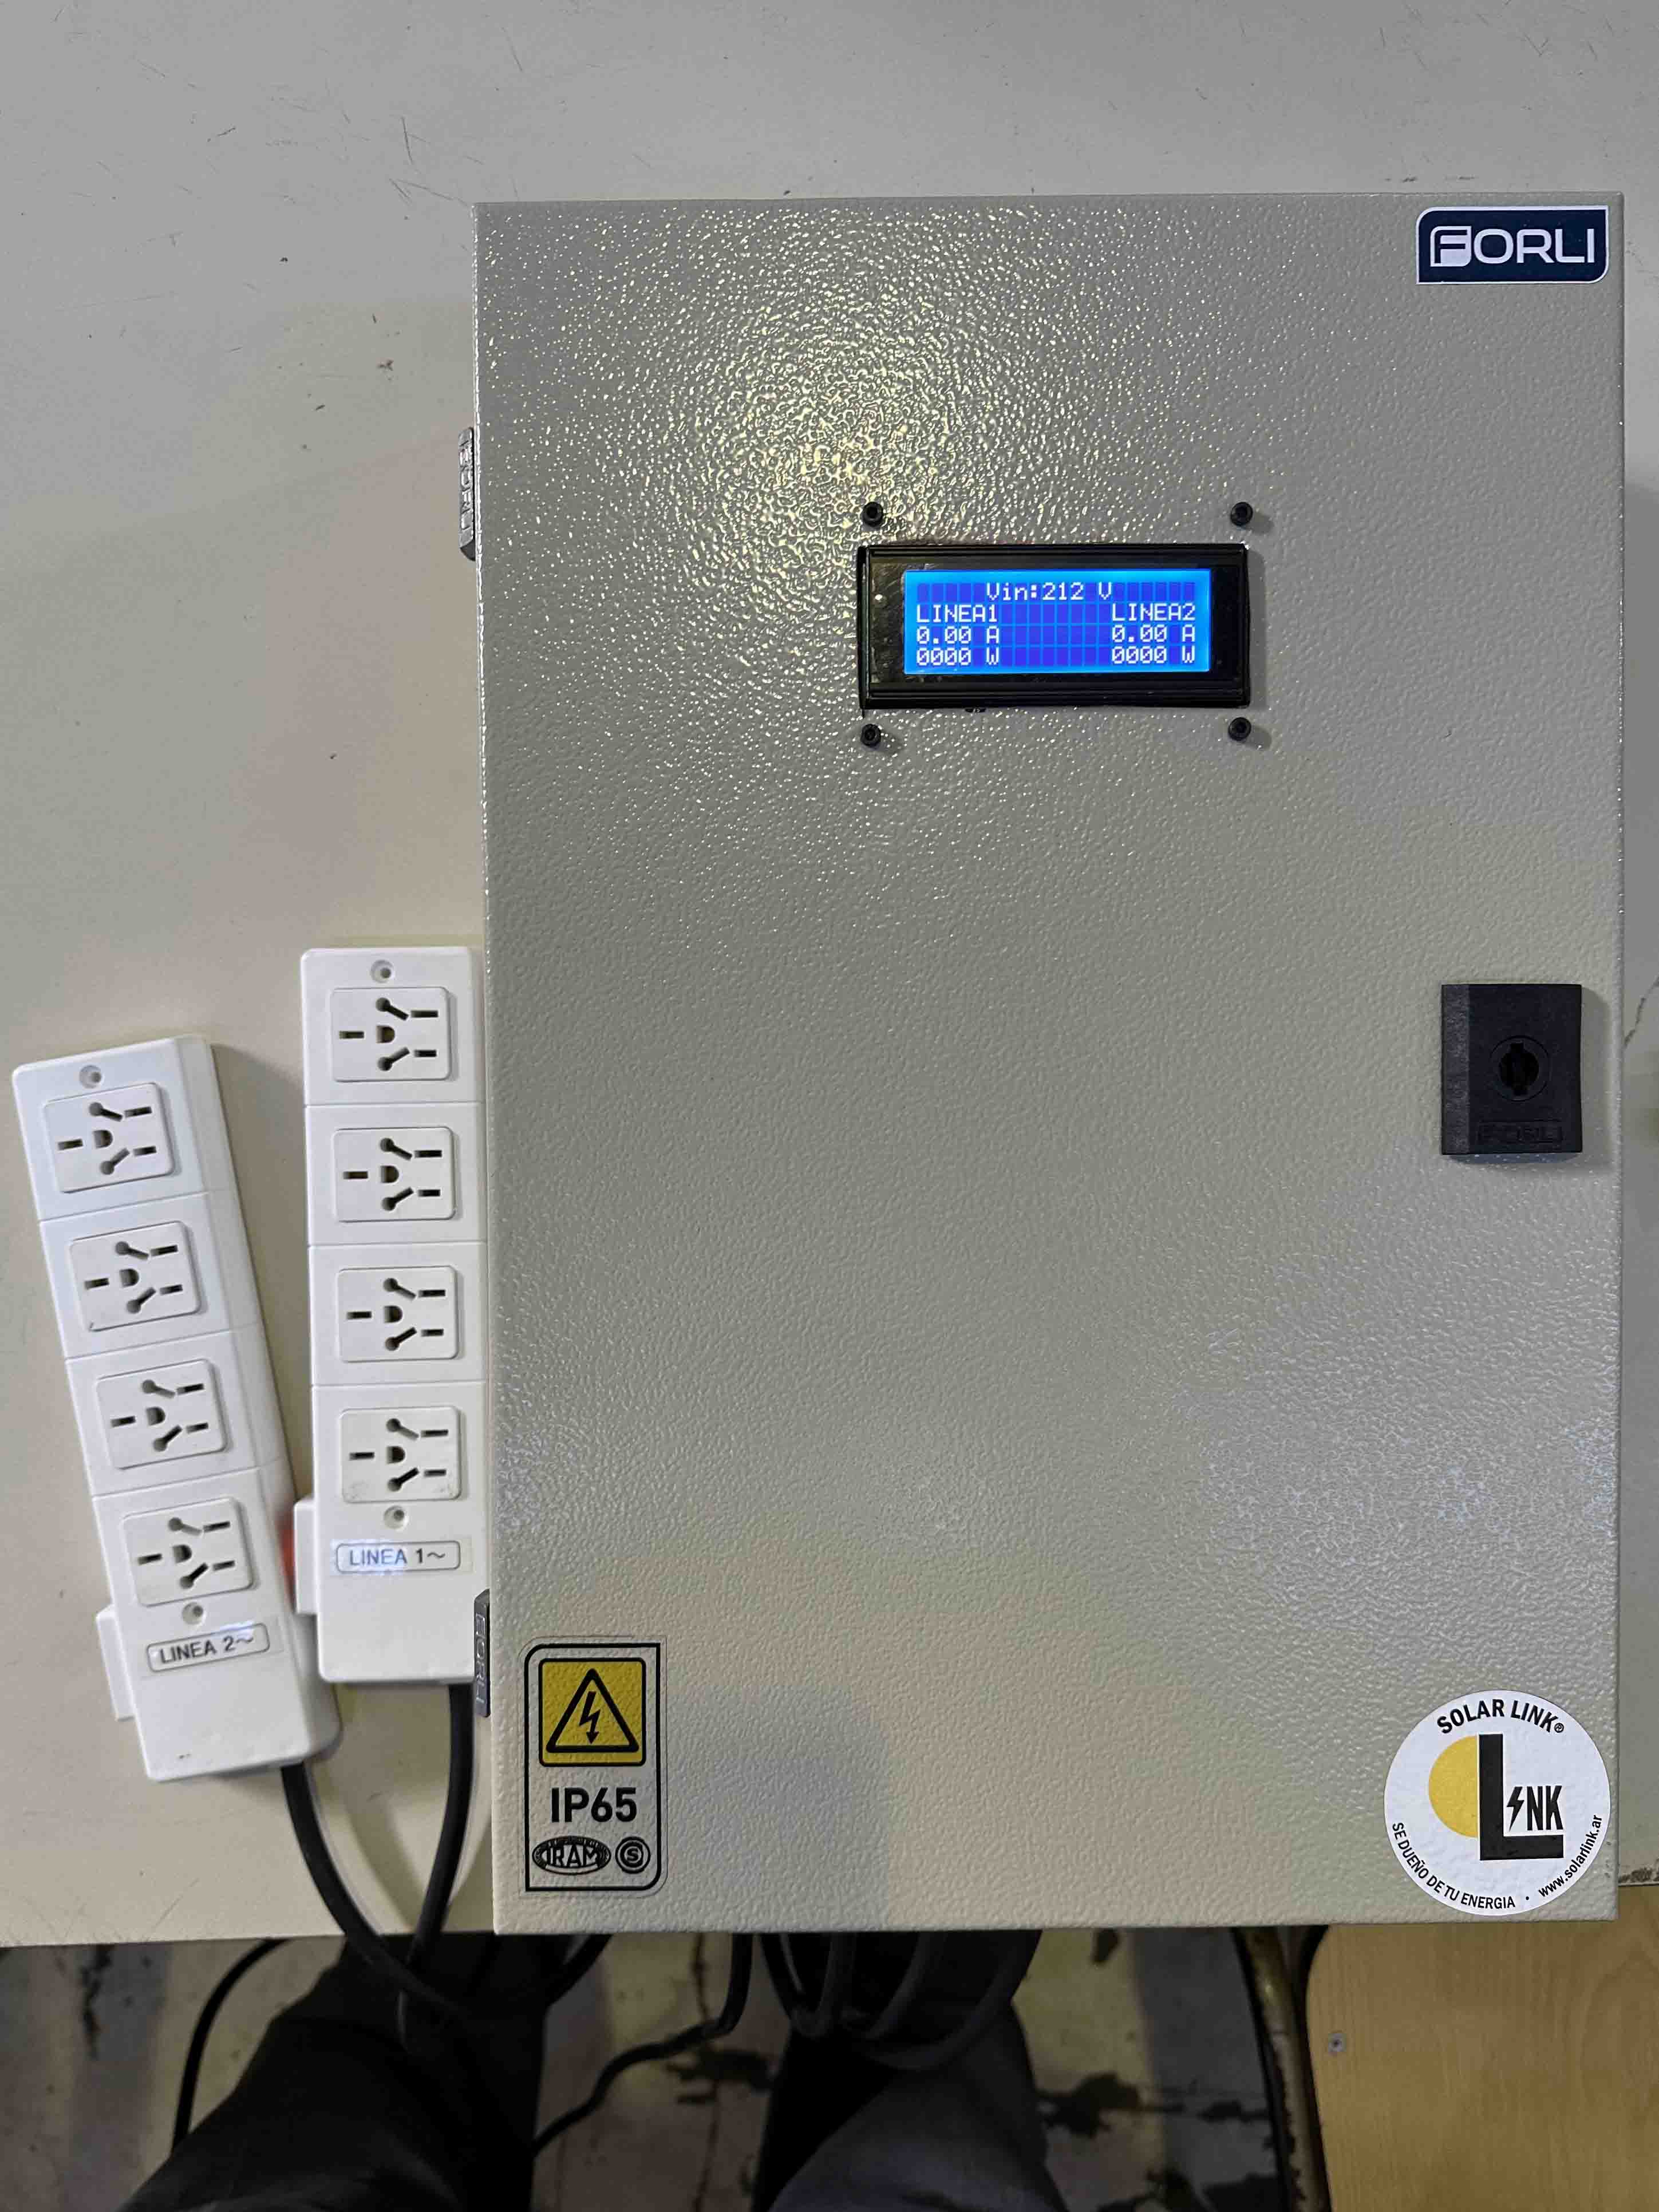
\includegraphics[width=0.9\linewidth]{proto-final/IMG_9418.jpg}
    \caption{Prototipo final de Solar Link.}
    \label{fig:final}
\end{figure}

\begin{figure}[H]
    \centering
    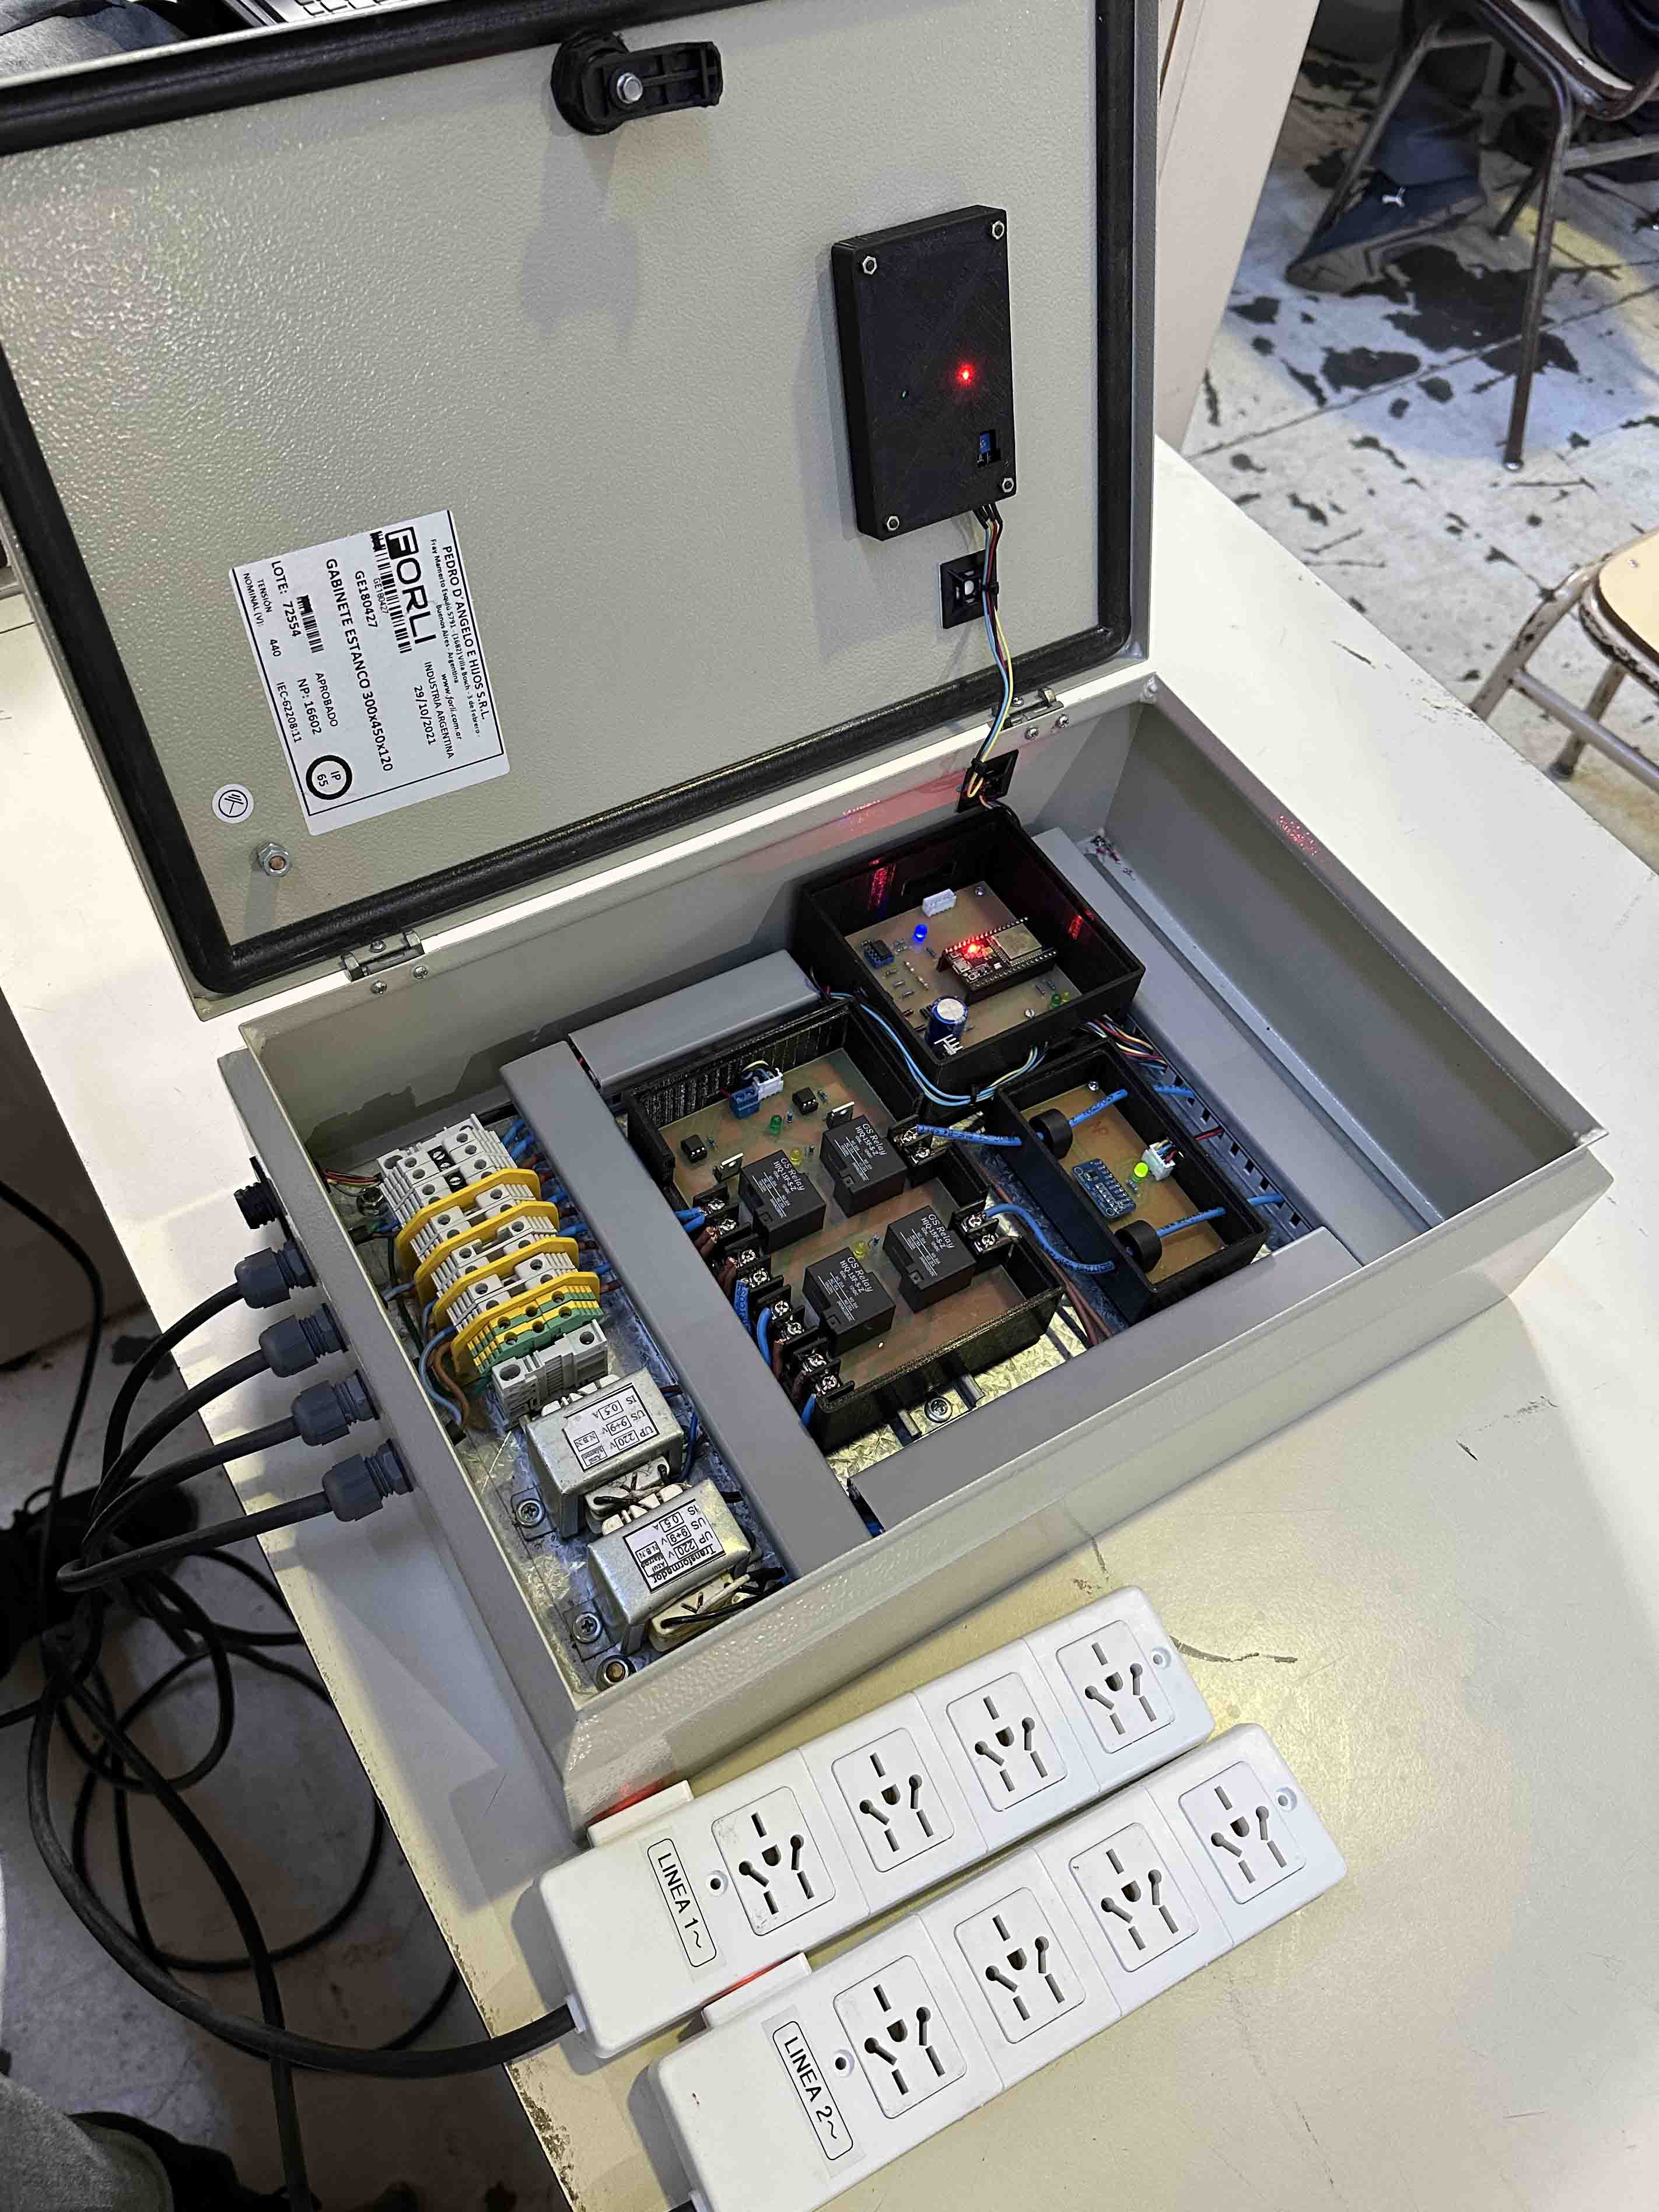
\includegraphics[width=1\linewidth]{proto-final/IMG_9419.jpg}
    \caption{Prototipo final de Solar Link por dentro.}
    \label{fig:final-in}
\end{figure}

Para la presentación final de Solar Link, desarrollamos el módulo de Solar Link, el cargador MPPT de 3 etapas, y un sistema solar off-grid completo.\\

El sistema off-grid, está compuesto por tres paneles solares, de 20W, 40W, y 70W, con una potencia total de 110W, una batería de 12V 240Ah, y un inverter de 2000W, ademas del cargador MPPT de 3 etapas.\\

\begin{figure}[H]
    \centering
    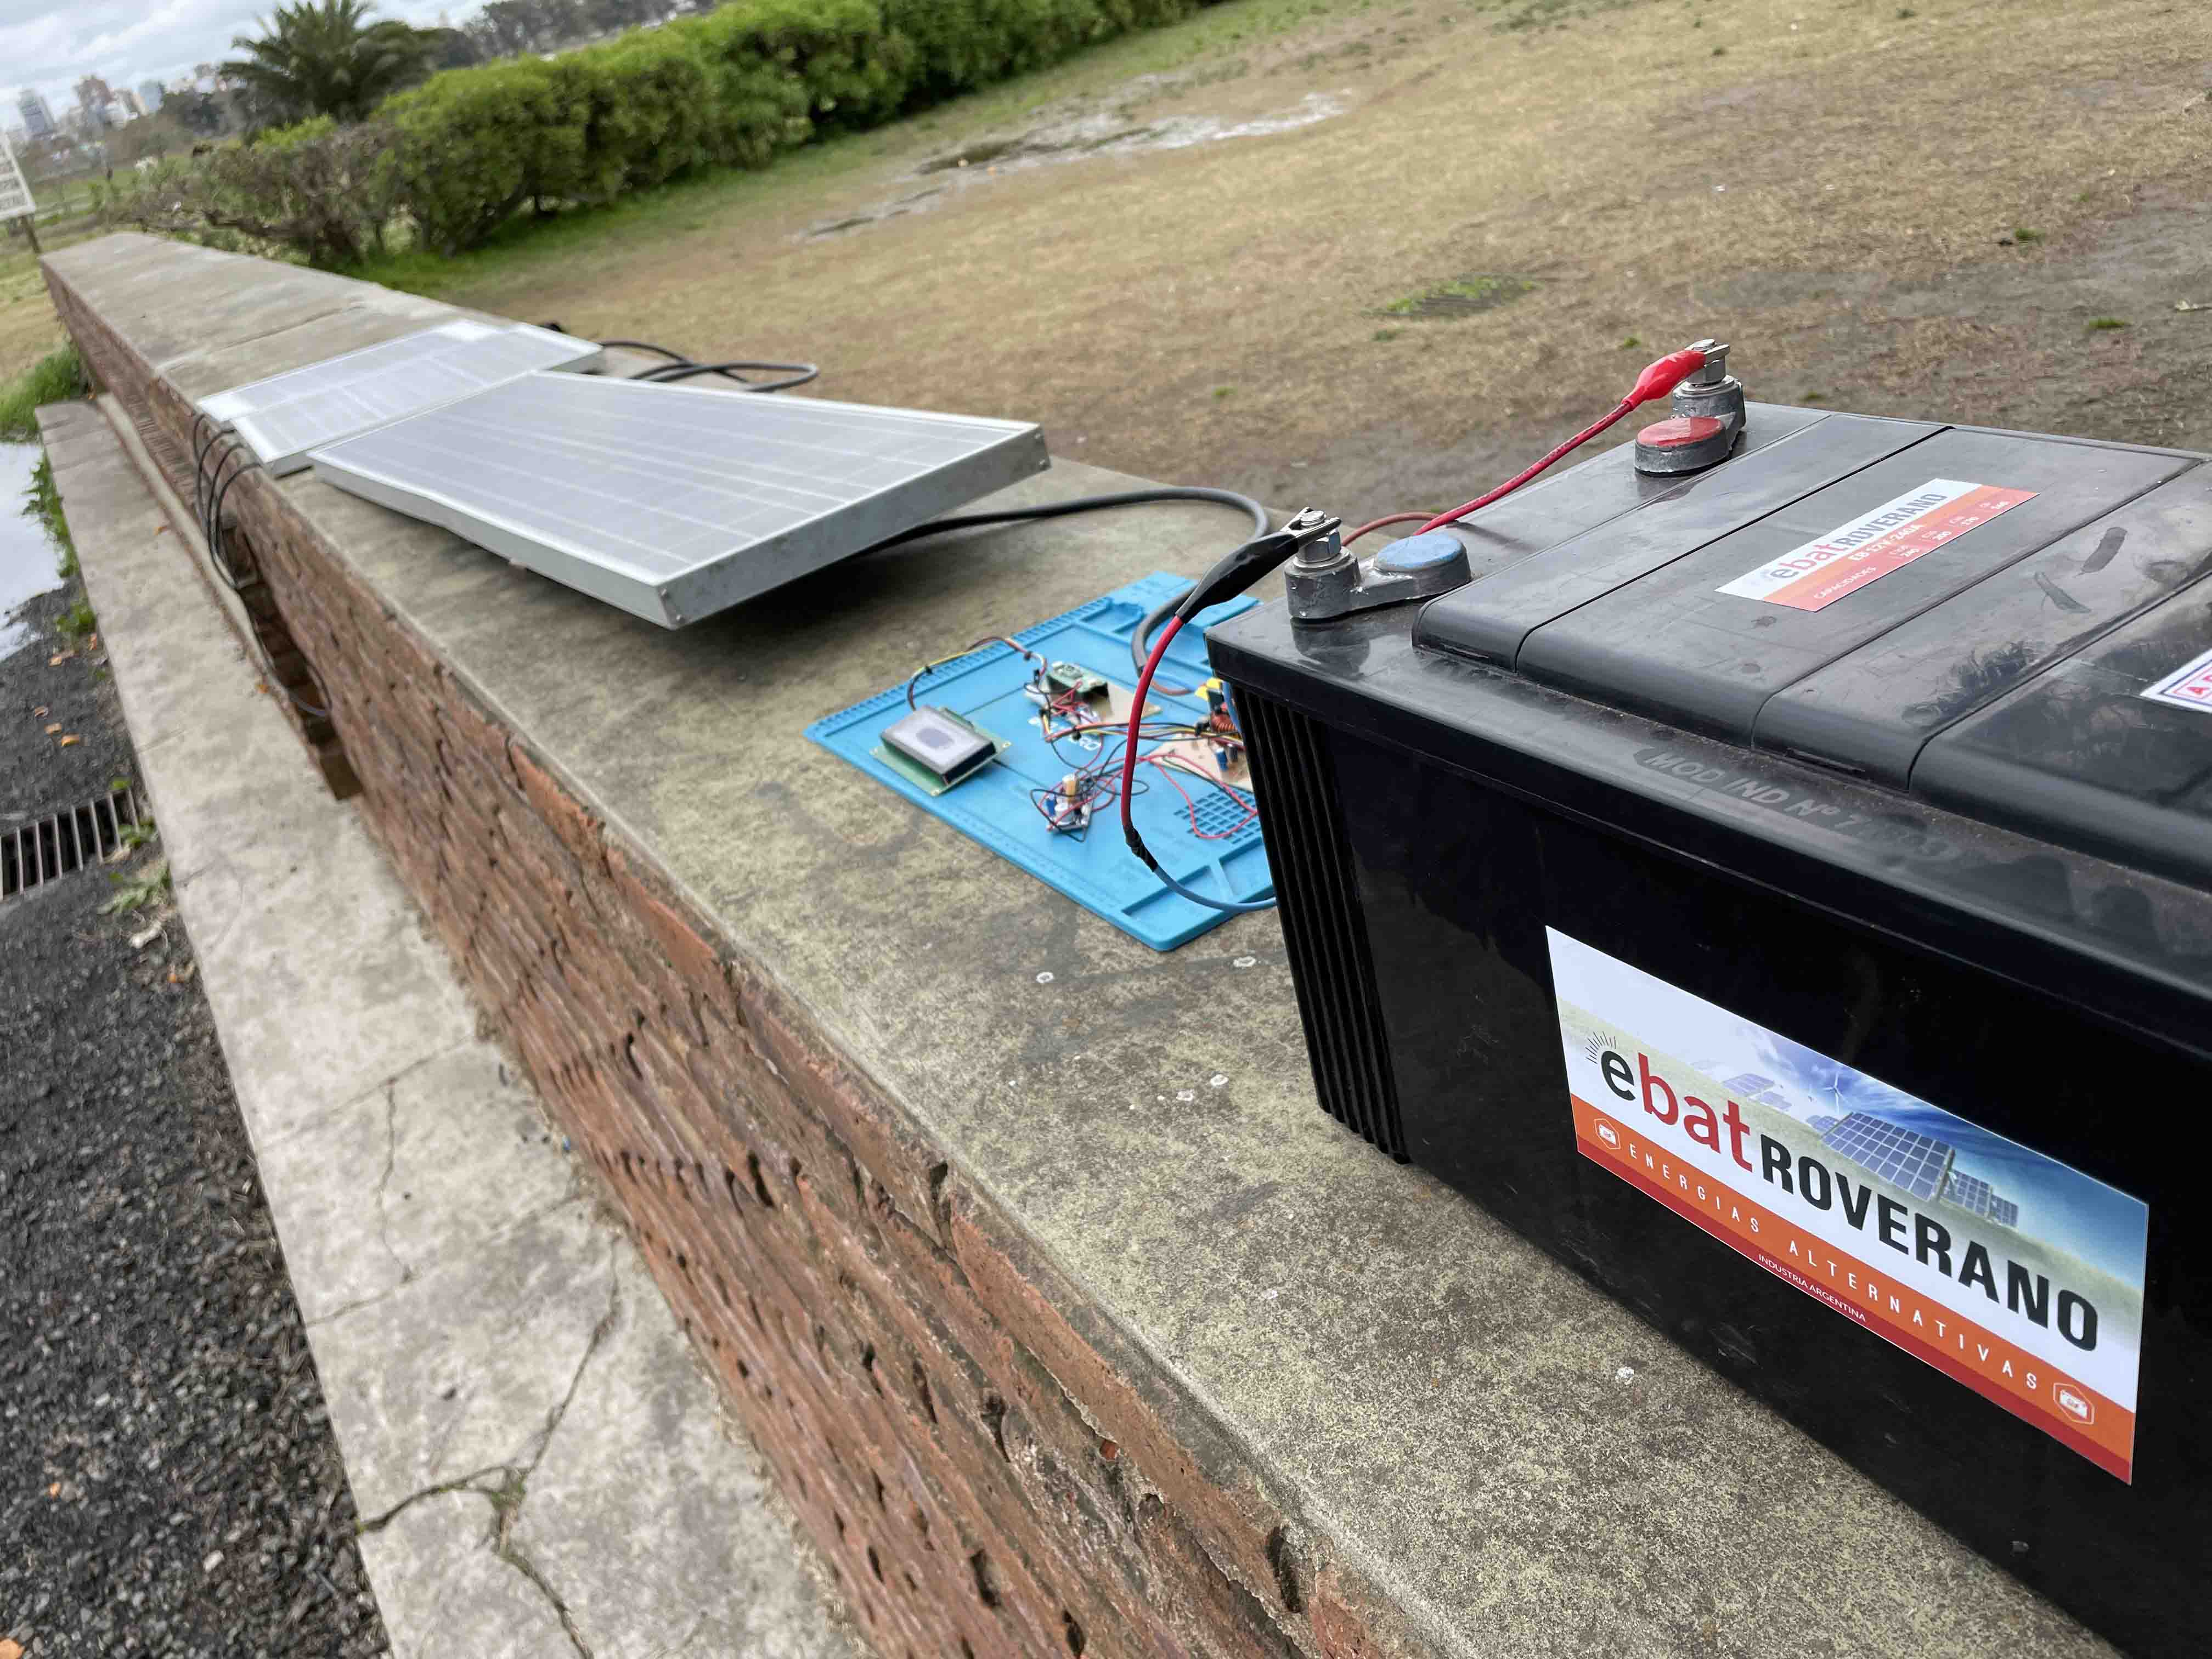
\includegraphics[width=1\linewidth]{proto-final/IMG_8911.jpg}
    \caption{Sistema off-grid en funcionamiento.}
    \label{fig:off-grid}
\end{figure}

\subsection{Conclusiones}

En las 32 semanas que duró el desarrollo de este proyecto, se lograron cumplir todos los objetivos que nos propusimos en un principio: realizar un producto y un servicio que le brinde al usuario beneficios energéticos, y que este sea capaz de acceder a toda la información sobre estos beneficios.\\

Nuestro administrador de energías renovables demostró que se puede acceder a este tipo de energías en un hogar argentino común y corriente sin una inversión inicial excesiva, ayudando al medio ambiente y al bolsillo de cada usuario.\\

La aplicación desarrollada es uno de los tantos puntos altos de este proyecto. Cada usuario con un Solar Link puede acceder desde cualquier dispositivo para monitorear todos los parámetros de consumo de su hogar.\\

Si bien no era uno de los objetivos iniciales, tambien pudimos desarrollar el cargador MPPT de 3 etapas, que nos permite darle a una batería una carga optimizada y saludable para su vida útil. Además, con el mismo objetivo que nos propusimos para Solar Link, le brinda al usuario toda la información posible, mostrándola tanto física como virtualmente.\\

Para finalizar, el desarrollo de este proyecto nos permitió a todo el grupo acceder a conocimiento que antes no poseíamos, que consideramos que es lo más importante. Toda la experiencia que conllevó el desarrollo de este proyecto será muy útil para lo que queramos seguir haciendo en el futuro.\\

\subsection{Mejoras a futuro}

Uno de los principales desperfectos del proyecto se encuentra en los relés inversores. Al ser estos mecánicos, al momento de la conmutación hay un punto muerto donde la línea de la casa no está alimentada, lo que puede llegar a dañar algunos electrodomésticos. La solución para esto es cambiarlos por relés en estado sólido, cuya conmutación se realiza casi instantáneamente. La desventaja de estos es su elevado precio y que no existen inversores, por lo tanto en lugar de 4 habría que utilizar 8 con una lógica externa, encareciendo mucho el producto final, pero siendo algo necesario al fin y al cabo.\\

Otras mejoras posibles se pueden realizar al cargador MPPT. Para utilizar diferentes tipos de baterías, es necesario reprogramarlo para cambiarle los parámetros internos de funcionamiento para la corriente de carga bulk, lo que conlleva tener que tener acceso al programa completo y a una computadora apta para esto. La solución para este problema es colocar una llave selectora en el exterior de este, la cual tenga varias corrientes, y el usuario pueda elegir la que mejor se adapta a su batería.\\

Además, a modo de protección, se puede utilizar un sensor de temperatura en la zona del disipador. Esto evitaría que se dañe el hardware en caso de una falla del sistema.\\

Por último, se podría migrar el programa del ESP32 de micropython a C, siendo un lenguaje de programación mas robusto puede evitar fallas en el funcionamiento.\\ 

\subsection{Especificaciones}
Administrador de energías renovables microcontrolado.

\begin{itemize}
    \item Voltaje de entrada de línea mínimo: 180Vac, 50Hz
    \item Voltaje de entrada de línea máximo: 240Vac, 50Hz
    \item Corriente de entrada de línea máximo: 10A
    \item Voltaje de entrada de energía solar mínimo: 180Vac, 50Hz
    \item Voltaje de entrada de energía solar máximo: 240Vac, 50Hz
    \item Corriente de entrada de energía solar máximo: 10A
    \item Voltaje de salida mínimo: 180Vac, 50Hz\
    \item Voltaje de salida máximo: 240Vac, 50Hz
    \item Corriente de salida máxima: 10A
\end{itemize}